\chapter{Cenni di Meccanica classica}
\label{meccanica_classica}
%\myChapter{Cenni di Meccanica classica}
\section*{Cinematica}
La Cinematica\cite{Douglas_classical_mechanics} � lo studio del moto di corpi materiali, senza considerare le cause e conseguenze di tale moto. La parte della Meccanica che si occupa delle cause e conseguenze del moto dei corpi � la Dinamica o Cinetica. La Cinematica fornisce una descrizione geometrica dei possibili moti.\\
Il soggetto mediante il quale vengono condotti gli studi in Cinematica � la particella, vale a dire un corpo immaginario, che occupa un singolo punto dello spazio. Un insieme di particelle le cui distanze relative rimangono invariate in ogni riferimento spaziotemporale. 

\subsection*{Moto rettilineo di una particella}


Le quantit� principali di cui si occupa sono
\subsubsection*{Posizione} Il vettore posizione della particella $P$ nel punto $A$: $\mathbf{r} = (x_A,y_A,z_A)$ con magnitudine $|\mathbf{r}| = \sqrt{x_A^2 + y_A^2 + z_A^2}$ $(m)$.

\subsubsection*{Spostamento} Lo spostamento da $A$ a $B$ di $P$: $\mathbf{r}_{AB} = \mathbf{r}_{B} - \mathbf{r}_{A}$ $(m)$

\subsubsection*{Distanza} La distanza $\displaystyle s=\int_{t_1}^{t_2}{\sqrt{\Big(\dfrac{dx}{dt}\Big)^2 + \Big(\dfrac{dy}{dt}\Big)^2+ \Big(\dfrac{dz}{dt}\Big)^2}dt}$ $(m)$ dove $t$ � il tempo. 


\subsubsection*{Velocit�} La \textbf{velocit�}
	\begin{itemize}
		\item \textbf{media} $\mathbf{\bar{v}} = \dfrac{\Delta \mathbf{r}}{\Delta t}$ $(m/s)$ con $\Delta t > 0$ 
		\item \textbf{istantanea} $\mathbf{v} = \displaystyle \lim_{\Delta t \rightarrow 0} \dfrac{\Delta \mathbf{r}}{\Delta t}$ con magnitudine $|\mathbf{v}| = \dfrac{ds}{dt}$ $(m/s)$
	\end{itemize}
	
\begin{figure}[h]
	\centering
		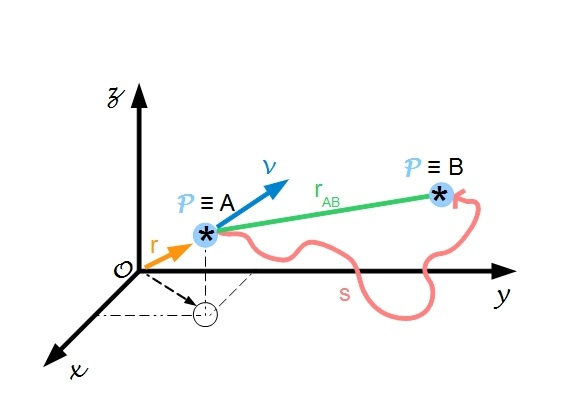
\includegraphics[width=.80\textwidth]{imgs/CinematicaLineare.jpg}
	\caption{Moto Rettilineo di una particella}
	\label{fig:CinematicaLineare}
\end{figure}
	
\subsubsection*{Accelerazione}
L'accelerazione
	\begin{itemize}
		\item \textbf{media} $\mathbf{\bar{a}} = \dfrac{\Delta \mathbf{v}}{\Delta t}$ con $\Delta t > 0$ $(m/s^2)$
		\item \textbf{istantanea} $\mathbf{a} = \displaystyle \lim_{\Delta t \rightarrow 0} \dfrac{\Delta \mathbf{v}}{\Delta t}$ $(m/s^2) $
	\end{itemize}
	
	

\section*{Moto Angolare di una particella}
\subsubsection*{Posizione} Il vettore posizione della particella $P$ nel punto $A$ rispetto ad un asse di rotazione $O-z$ �  $\mathbf{r}(t)$. La posizione angolare del punto $P$ � $\mathbf{r}_{\perp}(t) = r_{\perp x} \cos \theta i + r_{\perp x} \sin \theta j $ $(rad)$


\subsubsection*{Velocit�} 
La velocit� angolare � data da: 
		$\omega = \dfrac{d\theta}{dt}$ $(rad/s)$
	\begin{figure}[h]
	\centering
		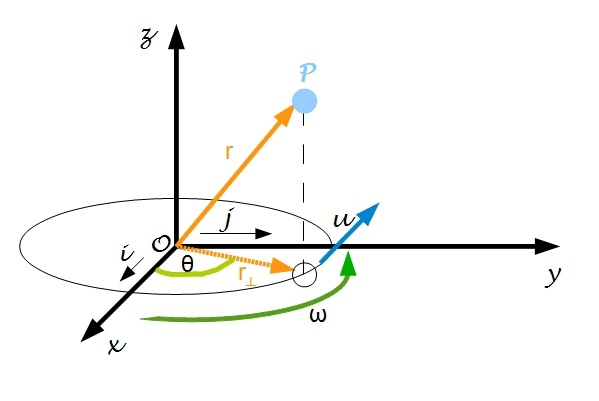
\includegraphics[width=.80\textwidth]{imgs/CinematicaAngolare.jpg}
	\caption{Moto Angolare di una particella}
	\label{fig:CinematicaAngolare}
\end{figure}
	
\subsubsection*{Accelerazione}
L'accelerazione angolare � data da:
	$\alpha = \dfrac{d\omega}{dt}$ $(rad/s^2)$
	
	
\section*{Dinamica (Cinetica)}
Branca della meccanica che si occupa di forze che producono, arrestano o modificano il moto di corpi. 
Le due leggi fondamentali della Dinamica sono quelle di Newton, in particolare la seconda:
\begin{equation}
F = ma
\label{eq:secondoPrincipioNewton}
\end{equation}